\documentclass[FM]{tulthesis}
% tento dokument používá balíky specifické pro XeLaTeX a lze jej přeložit
% jen XeLaTeXem, nemáte-li instalována použitá (komerční) písma, změňte
% nebo vymažte příkazy \set...font na následujících řádcích

\newcommand{\verze}{1.10}

\usepackage{polyglossia}
\usepackage{longtable}
\usepackage[toc,page]{appendix}
\usepackage{hyperref}	
\setdefaultlanguage{czech}
\usepackage{xevlna}


\usepackage{makeidx}
\makeindex

% appending
\appendixpageoff
%\appendixtitleoff

% fonty
\usepackage{fontspec}
\usepackage{xunicode}
\usepackage{xltxtra}
\usepackage{amsfonts}
\usepackage{graphicx}
\usepackage{float}
\usepackage{enumitem}
%\setmainfont[Mapping=tex-text,BoldFont={* Bold},Numbers=OldStyle]{Baskerville 10 Pro}
%\setsansfont[Mapping=tex-text,BoldFont={* Bold},Numbers=OldStyle]{Myriad Pro}
%\setmonofont[Scale=MatchLowercase]{Vida Mono 32 Pro}

% příkazy specifické pro tento dokument
\graphicspath{ {./images/} }
\newcommand\litem[1]{\item{\bfseries #1 -}}
\newcommand{\argument}[1]{{\ttfamily\color{\tulcolor}#1}}
\newcommand{\argumentindex}[1]{\argument{#1}\index{#1}}
\newcommand{\prostredi}[1]{\argumentindex{#1}}
\newcommand{\prikazneindex}[1]{\argument{\textbackslash #1}}
\newcommand{\prikaz}[1]{\prikazneindex{#1}\index{#1@\textbackslash #1}}
\newenvironment{myquote}{\begin{list}{}{\setlength\leftmargin\parindent}\item[]}{\end{list}}
\newenvironment{listing}{\begin{myquote}\color{\tulcolor}}{\end{myquote}}
\sloppy

% \textbf{ pro titulní stránku
\TULtitle{Java pro ztracené případy}{Java for lost causes}
\TULprogramme{B0613A140005}{Informační technologie}{Information technology}
\TULbranch{B0613A140005IT}{Informační technologie}{Information technology}
\TULauthor{Kevin Daněk}
\TULsupervisor{ - }
\TULyear{2022}
\TULthesisType{Semestrální práce}{Semestral work}

\begin{document}

	
	\ThesisStart{male}
	%\ThesisStart{zadani-a-prohlaseni.pdf}
	\begin{abstractCZ}
	Práce se snaží jednoduchými metaforami a analogiemi uvést čtenáře do problematiky programování, konkrétně programování v objektově orientovaném jazyce Java.
\end{abstractCZ}


\begin{keywordsCZ}
	Java, návod, programování, objektově orientované programování, základy programování
\end{keywordsCZ}

\vspace{2cm}

\begin{abstractEN}
	This document is trying to explain fundamental programming concepts through simple analogies and metaphores reflecting the real life scenarios. It's main focus is explaining the problem of creating an algorithm and expressing it through structural and object oriented programming patterns.
\end{abstractEN}

\begin{keywordsEN}
	Java, guide, programming, object oriented programming, programming fundamentals
\end{keywordsEN}

\begin{acknowledgement}
	Děkuji lidem, co si tohle opravdu přečetli.
\end{acknowledgement}
	\clearpage

	\tableofcontents	
	\listoffigures
	\listoftables
	
	\chapter{Úvod}
Tato práce se zaobírá problematikou programování, a to konkrétně obecné algoritmizace a lehkého úvodu do OOP. Kvůli omezení rozsahu je odstraněna Java část a kus OOP části.

V textu nejsou jednotlivé pojmy explicitně definovány, proto jsou definice jednotně uvedeny ve \hyperref[app:slovnik]{slovníku}, který naleznete v příloze.
	\chapter{Úvod do programování a algoritmizace}
\section{Programování a algoritmizace}
Pod programováním si spousta lidí představí spoustu věcí - kdybych ale měl tento pojem popsat jednou větou, asi bych ho popsal nějak takto:

Ačkoliv né uplně přesná definice, podle mého názoru dává nejlepší představu o tom, co programování vlastně je. Programování je o hledání řešení nějakého problému, jak toto řešení vyjádřit a zajistit, aby řešení bylo co nejvhodnější danému problému. Programování už z výše uvedené definice říká, že vede k nějakému postupu, který daný problém řeší. Tento postu označujeme honosným názvem "\textbf{algoritmus}".

Nejčastěji se setkávám s přirovnáním ke kuchařce, proto si ho dovolím použít i zde: Za algoritmus můžeme považovat recept, kde máme přesnou sadu instrukcí, které nám říkají, jak něco uvařit. Tenhle recept vždy vede ke stejnému výsledku (nemůže se nám stát, že pomocí receptu na koprovku uděláme rajskou, že ano) a vždy bude doba vaření trvat stejně dlouho.

Už jenom z této intuice můžeme odvodit některé vlastnosti algoritmů:
\noindent
\begin{enumerate}
	\litem{Obecnost} Algoritmus by měl být dostatečně obecný na to, aby dokázal řešit pokud možno co nejvíce případů.
	\litem{Determinovanost} Výsledek algoritmu by měl být předvídatelný.
	\litem{Konečnost} Algoritmus musí v nějakém bodě skončit.
	\litem{Srozumitelnost} Algoritmus by měl dávat smysl a nemělo by být zbytečně složité ho pochopit.
	\litem{Efektivita} Algoritmus by neměl plýtvat zdroji a být pokud možno co nejúspornější. To samé platí i o čase potřebném na jeho vykonání.
\end{enumerate}

Tato pětice bodů je kolektivně známa jako \textbf{vlastnostni algoritmu}. Ovšem jak takový algoritmus vytvoříme? Proces takzvané \textbf{algoritmizace} by se dal popsat v následujících krocích:
\begin{enumerate}
	\litem {Analýza zadání} Pořádně se podíváme, co se po nás a našem algoritmu chce.
	\litem {Rozložení na menší problémy} Pokud je původní zadání komplexnější, rozložíme si ho na několik menších problémů, které budeme postupně řešit
	\litem {Návrh řešení} Rozmyslíme, jakými způsoby můžeme dílčí problémy řešit, a který postup by byl pro nás nejlepší.  
	\litem {Zápis algoritmu}  Algoritmus zformulujeme a zapíšeme
	\litem {Ladění} Algoritmus zkontrolujeme, zda se chová tak, jak má.
\end{enumerate}
Výsledkem této algoritmizace bude konečný sled kroků, který můžeme následně použít k vytvoření programu. Jak ale takový algoritmus zapíšeme? 

Metod je spousta, a jsou to asi takové, které by vás napadly. Můžeme algoritmus vyjádřit slovně, písemně po větách, v programovacím jazyce nebo pomocí vývojových diagramů. Hlavně poslední způsob zápisu je velmi oblíbený ve školách na otravování studentů, proto se ním tady zabývat nebudu.

Na závěr téhle kapitoly bych vám rád ukázal diagram níže, který propojuje všechny výše zmíněné pojmy dohromady a jak vlastně spolu souvisí:
\begin{figure}[H]
	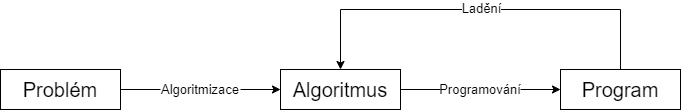
\includegraphics[width=\textwidth]{programovani_algoritmizace}
	\centering
	\caption{Diagram tvorby programu}
\end{figure}

\subsection{Asymptotická složitost algoritmů}
Vzpomeňte si zpátky na \textbf{vlastnosti algoritmu} - jednou z nich byla \textbf{efektivita}. Jak ale určíme, co je "dostatečně dobrá" efektivita, a co ne? Ačkoliv to nejde přímo univerzálně určit, protože to vždy záleží na dané situaci, ale z matematiky si můžeme vypůjčit nástroj, který nám dovolí zhruba určit, jak dlouho bude nějaká operace trvat. Tomuto nástroji se říká \textbf{asymptotická složitost} nebo také \textbf{Big O Notation}.

\begin{figure}[H]
	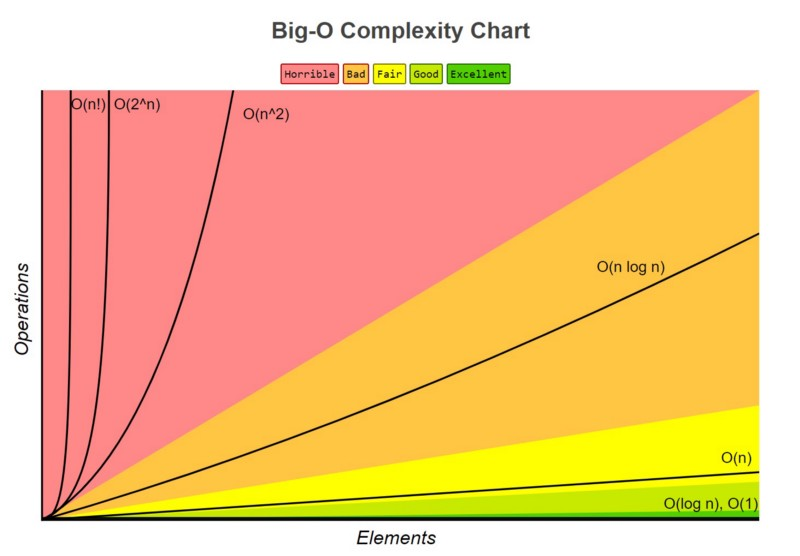
\includegraphics[width=\textwidth]{big_o_notation}
	\centering
	\caption{Graf asymptotických složitostí (freecodecamp.org)}
\end{figure}

Asymptotická složitost se určuje hlavně pro dvě domény:
\begin{enumerate}
	\litem {Časová složitost} Jak rychle roste čas potřebný na zpracování dat
	\litem {Paměťová složitost} Jak rychle roste paměť potřebná na provedení algoritmu
\end{enumerate}

Málo kdy se podaří mít optimalizovat jak čas, tak paměť (zpravidla bývá optimalizace jedné veličiny na úkor druhé). V dnešní době se spíše upřednostňuje optimalizace času, jelikož dostupné paměti je dnes docela dost.

Jak tedy takovou časovou asymptotickou složitost vypočítat? No, to je trochu složitější a je důležité říct, že je většinou spíše o odhady. Typ složitosti se dá zpravidla odhadnout z konkrétního kódu (například dvě vnořené smyčky do sebe mívají kvadratickou složitost). 

Pokud to ale nelze odhadnout, lze samozřejmě provést měření a určit jednu z funkcí, která nejlépe odpovídá nárustu v čase. Podívejte se na ilustrační obrázek níže - Na ose $x$ máme počet vstupních dat (z pravidla se používá logaritmické měřítko) a na ose $y$ čas, který byl potřeba na vykonání.

\begin{figure}[H]
	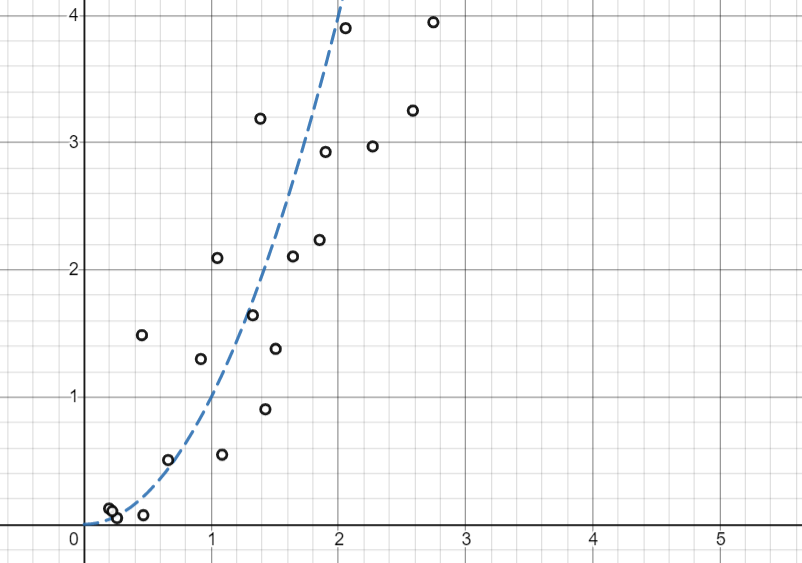
\includegraphics[width=\textwidth]{big_o_ukazka}
	\centering
	\caption{Ukázka proložení bodů z měření parabolou}
\end{figure}

Černé kroužky jsou body, které odpovídají naměřeným hodnotám, a modrá přerušovaná čára je pravá větev paraboly, kterou data prokládáme. Když se na takhle na tento obrázek podíváme, asi se shodneme, že hodnota bodů roste tak nějak podobně jako parabola, kterou jsme přidali.

S tímto závěrem bychom řekli, že funkce, která vytvářela tyhle body, má \textbf{kvadratickou časovou složitost}, nebo bychom zapsali v podobě O-notace $O(n^2)$.

Důležité si je uvědomit, že nám to neříká nic jiného, než jak čas roste v závislosti na objemu vstupních dat - nemá to být nějaký přesný výpočet - spíše jenom pomůcka k rychlému ohodnocení efektivity algoritmu.

\section{Datové typy}
Při programování pracujeme s daty různých typů - můžeme pracovat s celými čísly, reálnými čísly, s řetězci znaků a dalšími blbostmi. Datové typy programovacímu jazyku říkají, co za data chceme v proměnné ukládat, a respektive, jak je má ukládat v paměti.

Nejčastější a nejzákladnější datové typy jsou celá čísla (\textit{integers}), reálná čísla (\textit{doubles}), znaky (\textit{chars}) a textové řetězce (\textit{strings}).

Občas se ale může stát, že máme data uložena v jednom datovém typu, například řetězci znaků, a potřebujeme s ním pracovat jako s jiným typem, například číslem. To se stává často u zpracování uživatelského vstupu, který bývá celý uložen v řetězci znaků (\textit{string}) \cite{kralovcova}. Když chceme po uživateli zadat čísla, dostaneme akorát znaky, a my si musíme poradit. Pokud chceme z řetězce znaků dělat číslo, přichází na řadu proces \textbf{přetypování}.

Přetypování bývá velmi nebezpečný proces, který je často náchylný na vyvolání chyby. Proč? Představme si opět převod řetězce znaků na číslo. Při převodu mohou nastat 3 případy:
\begin{enumerate}
	\item V řetězci jsou jenom cifry, tudíž bude převod úspěšný
	\item V řetězci jsou cifry a nějaký další znak, s trochou štěstí dostameme akorát to číslo, v horším případě chybu
	\item V řetězci jsou znaky, které nelze přeložit na číslo. Buďto se vyvolá chyba, nebo se nám vrátí hodnota typu NaN.
\end{enumerate}

To jsou takové základní případy, které by mohly nastat. Může jich být více či méně, hodně záleží na samotných programovacích jazycích, jak moc se snaží běh programu zachránit. Některé při převodech chybu nevyvolají, ale pak musíme kontrolovat správnost převodu.

\section{Programovací paradigma}

Když vysvětluji, co je programovací paradigma svým kamarádům, rád říkám, že to je takový "styl programování" a přirovnávám to k zaklínačským školám z povídek Andrzeje Sapkowského (a respektive jejich videoherním adaptacím). 

Každá zaklínačská škola učí své zaklínače, jak se připravit na souboj, jak získat výhodu v boji a jak vůbec bojovat - zda být hbitý a mít výhodu rychlosti, či si držet půdu pod nohama a získat výhodu síly. Podobně je to i s programovacími paradigmaty, kde by každé paradigma odpovídalo bojovému stylu jiné zaklínačské školy.

Každé paradigma (styl) programování popisuje problém jinak, a tak vždy k výsledku dospěje jinou cestou, obecně je ale můžeme rozdělit na dvě velké kategorie:
\begin{enumerate}
	\litem{Imperativní} Zde říkáme, jaké kroky má program udělat, abychom dospěli ke chtěnému výsledku
	\litem{Deklarativní} Zde zase říkáme, co za výsledek chceme, a necháme program, ať se k němu nějak dopracuje.
\end{enumerate}

Nejčastěji se asi setkáte s jazyky \textbf{imperativními}, mezi které patří velká jména jako \textit{Java, C, C++, C\#, Rust, Python} a spousta dalších. Mezi \textbf{deklarativními} jazyky jsou také velká jména, ale jsou to jazyky spíše pro kontrolu nějakých rozhraní (například \textit{SQL} pro vytváření dotazů na databázi, či \textit{CSS} pro stylování webové stránky).

\section{Strukturované programování}

Strukturované programování je označení pro paradigma, které vzniklo z frustrace nad nestrukturovaným programováním, ve kterém bylo složité větvit program podle aktuálního stavu dat či opakovaně volat nějaký blok kódu. Ačkoliv je toto knížka o Javě, která je objektově orientovaná, připadá mi dobré zmínit základní struktury (viz tabulka \ref{table:strukturovane}), na kterých strukturované programování stojí, jelikož je objektově orientované programování v jistém slova smyslu nadstavbou ke strukturovanému.

Prvně si vysvětlíme rozdíl mezi \textbf{výrazem} a \textbf{příkazem}, a co je to \textbf{operátor}. Základním rozdílem mezi výraz a příkazem je tedy to, že výraz je vyhodnocován, a příkaz vykonáván. Operátory znáte běžně z matematiky, jedná se například o plus, mínus, krát či děleno. Operátory se ovšem ještě podle svojí funkce dají dále dělit na:

\begin{enumerate}
	\litem{Aritmetické} To jsou operátory jako $+, -, \cdot, /$
	\litem{Logické} Tyhle operátory určují logický vztah mezi levou a pravou stranou, například AND, OR, NOT, a jejich kombinace.
	\litem{Relační} Tyhle operátory určují vztah mezi hodnotami, například $<, \le, =, >, \ge$
\end{enumerate}

S výrazy, příkazy a operátory jsme nyní schopni popsat spoustu problémů. Stále zde ale máme jisté techniky a principy, které popisování problému razantně usnadňují.

\begin{table}[h!]
	\caption{Hlavní rysy strukturovaného programování}
	\label{table:strukturovane}
	\begin{tabular}{|m{0.4\linewidth} | m{0.6\linewidth} |}
		\hline
		Sekvenční zpracování instrukcí & Instrukce se vykonávají v pořadí tak, jak jsou zapsané od zhora dolů               \\ \hline
		Funkce a procedury             & Blok kódu, pomocí kterého můžeme jednou instrukcí spustit vícero vnořených příkazů \\ \hline
		Větvení programu               & Rozdělení běhu programu podle logické podmínky                                     \\ \hline
		Cykly                          & Pro opakované vykonávání instrukcí                                                 \\ \hline
	\end{tabular}
\end{table}

\section{Datové struktury}
Když se podíváme na nadpis téhle kapitoly, možná vás již napadne, že datové struktury budou něco, co nám pomůže nějakým způsobem strukturovat data. A divte se nebo ne, měli byste pravdu. Stejně jako \textbf{datové typy} říkaly, jak hodnoty ukládat v paměti, \textbf{datové struktury} nám zase říkají, jak ukládat vícero hodnot v paměti.

Tou nejprimitivnější datovou strukturou je \textbf{pole}, které najdete prakticky v každém programovacím jazyce. Pole je velmi dobré znát, jelikož díky němu dokážete vytvořit další datové struktury\footnote{Ono je to trochu složitější - lze s nimi tyto struktury vytvořit, ale né vždy budou moci konkurovat jejich nativním implementacím.}.

Pole má jednu zásadní nevýhodu, a to je jeho fixní délka. Tento problém řeší datová struktura \textbf{list} (nebo také známo jako \textbf{seznam}), jejíž délku lze libovolně rozšiřovat či zmenšovat - její nevýhodou je však větší (a tím pádem i časově náročnější) režie s pamětí\footnote{Ono ani tohle není úplně pravda - rozhodně zabírá více místa v paměti, ale pak už záleží na implemetaci (např. zřetězení prvků pomocí odkazů na další prvek má režii minimální)}.

Další obecnou datovou strukturou je \textbf{asociativní pole} (též známo jako \textbf{mapa} nebo \textbf{slovník}). Tahle struktura dále staví na konceptu \textit{pole} a rozšiřuje možnosti, jak přistupovat k prvkům. K polím přistupujeme pomocí celočíselných indexů, v asociativním poli ale můžeme používat místo celočíselného indexu takzvaný \textit{klíč}. 

Příkladem může být např. jazykový slovník, kde klíčem je cizí slovíčko, a hodnotou je český překlad. Nebo třeba telefonní seznam, kde klíčem je jméno člověka, a hodnotou je telefonní seznam\footnote{Nebo naopak. Zpravidla jsou asociativní pole jednoznačná, takže lze vytvářet inverze a z hodnot udělat klíče a naopak}.

\section{Výjimky a chybové stavy}
Bohužel nastávají situace, kdy naše programy mohou \textit{zpanikařit}. Představme si program, který se chová jako jednoduchá kalkulačka s reálnými čísly a klasickými aritmetickými operacemi. No a teď si představme, že do ní nějaký matlák\footnote{Čtěte jako matlabák} nacvaká $\frac{1}{0}$. Nulou v reálných číslech dělit neumíme, takže, co teď? Zpravidla by program takzvaně \textit{vyhodil} či \textit{vyvolal} \textbf{výjimku}. 

Výjimkou tak vyvolá například již výše zmíněné dělení nulou, nebo třeba čtení neexistujícího souboru. Výjimky jsou takto pojmenované právě kvůli tomu, že se jedná o \textit{výjimečné stavy} programu, a programovací jazyky nám dávají možnost tyto stavy ošetřit a program \textit{zotavit}. Nad výjimkou ovšem stojí ještě \textbf{chybový stav}.

Chybou může být například špatné přidělování paměti či chyba způsobená nižším rozhraním. Takovým typickým příkladem chybového stavu ze života je \textit{modrá obrazovka smrti}. Z chyb se program kvůli jejich vážnosti nezotavuje - prakticky by to ani nebylo možné.
	\chapter{Úvod do objektového programování}
Objektově orientované programování (dále už jenom OOP) je jedno z nejrozšířenějších programovacích paradigmat. Nachází velké rozšíření napříč programovacími jazyky a je de-facto jedním z nejpoužívanějších paradigmat. Jeho výhodou je rozhodně jednoduchost návrhu řešení problému - OOP se totiž snaží simulovat reálný svět tím, že problém popíše pomocí různých entit, které mezi sebou navzájem interagují a dohromady řeší problém. Je to velmi podobné například manufaktuře, kde každý pracovník dělá jenom konkrétní činnost, jejíž výsledek poté předává dál - a na konci pak čeká již hotový výrobek.

Ačkoliv je OOP velmi jednoduchý na pochopení, tak je také velmi jednoduchý na pokažení. OOP se dokáže velmi zvrtnout, velmi rychle. Jsou také případy, kdy OOP nepřináší žádnou výhodu a jiné paradigma by možná bylo užitečnější - to už pak záleží na zdrojích, které nám poskytuje konkrétní programovací jazyk.

Nenechte se tímto odradit, jenom jsem chtěl upozornit na to, že OOP není blbuvzdorné a může vám v případě špatného použití spíše zavařit než-li pomoci.

\section{Objekty}
Základním stavebním blokem objektově orientovaného programování je, jak už název napovídá, \textbf{objekt}. Jako objekt se v objektově orientovaném programování označuje ledacos, a je to pojem spíše nápomocný k vysvětlování dalších pojmů. My budeme chápat jako objekt strukturu, která si uchovává dvě podstatné věci:

\begin{itemize}
	\item \textbf{Data} - Informace a hodnoty, se kterými může objekt nějak pracovat
	\item a \textbf{Operace} - Věci, které dokáže provést
\end{itemize}

Data a operace nejsou ovšem není zrovna správné pojmenování těchto věcí - častěji se setkáte s jejich odbornými termíny, což jsou \textbf{atributy} (data) a \textbf{metody} (operace). Každý z tento pojmů postupně probereme.

\subsection{Atributy}
Jako atributy označujeme proměnné nebo konstanty, ve kterých si objekt uchovává informace a hodnoty, které dále ve svém kódu využívá. Tyto atributy jsou nejčastěji používány buďto pro sdílení informací napříč jednotlivými metodami, nebo pro nastavování nějakého obecnějšího chování.

Představme si například objekt \textbf{obdélník}. Každý obdélník má \textbf{délku} a \textbf{šířku}. Délka a šířka jsou tedy atributy objektu obdélník. Tyto atributy můžeme dále používat pro výpočet obvodu, obsahu či úhlopříček...

\subsection{Metody}
Metody jsou operace, které může nějaký konkrétní objekt provádět. Jedná se konkrétně buďto o funkce nebo procedury, které má objekt k dispozici.

Metody jsou hnacím motorem daného objektu - slouží k dělání výpočtů, manipulaci s dalšími objekty, vytváření dalších objektů, zkrátka objektu dají nějakou funkcionalitu.

\section{Vytváření objektů a přístup k objektům}
Zatím jsme si popsali objekt jako takový, ale neřekli jsme, odkud se objekty berou. Aby programovací jazyk věděl, jakým způsobem má nějaký objekt vytvořit, potřebuje pro něj nějaký \textbf{předpis}. Tomuto předpisu se říká \textbf{třída}.

\subsection{Třída objektu}
Třída objektu předepisuje, jaké vlastnosti a metody bude daný objekt mít. Vzpomeňte si na naší definici objektu - je to věc, která si uchovává v paměti atributy a metody. Třída nedělá nic jiného, než že říká, co tyhle vlastnosti a metody jsou konkrétně zač.

S předpisem v ruce může programovací jazyk začít tvořit objekty - kde má ale začít? K tomu lze využít buďto již zabudovanou, nebo námi vytvořenou speciální metodu, které se říká \textbf{konstruktor}.

\subsection{Konstruktor a destruktor}
Konstruktor je metoda, kterou má každá třída, a která říká programovacímu jazyku, jak má vytvářet nové objekty. Každá třída má svůj tzv. \textit{implicitní konstruktor} - to je takový, který se použije, pokud tam nemáme svůj vlastní (respektive nazvaný \textit{explicitní konstruktor}).

Konstruktory se používají k naplnění objektu daty, které můžeme pomocí argumentů předat z vnějšího programu. Vždy je výsledkem konstruktoru nová instance objektu - zpravidla lze vytváření objektu pomocí konstruktory přerušit akorát vyvoláním výjimky. Existují principy, jak vytvářet objekty a případně zamezit jejich vytvoření, ale to je mimo rozsah této příručky. Analogicky k metodě, která vytváří objekt, také existuje metoda, která objekt níčí (Odborníci čtěte jako \textit{uvolňuje z paměti}). Té se říká \textbf{destruktor}.

\subsection{Modifikátory přístupu}
Jak už název napovídá, modifikátory přístupu \textit{modifikují přístup} - otázkou je, přístup k čemu modifikují? Odpovědí je tak nějak ke všemu.

Tahle definice se může zdát trochu vágní - vysvětlím tedy na příkladech. Nejdříve ale konkrétní modifikátory přístupu - nejčastěji se setkáte s dvojicí \textbf{public} a \textbf{private}. \textbf{Public} strukturu prezentuje celému zbytku programu, kde jakákoliv další struktura k němu má přístup, naopak \textbf{private} strukturu schová.

\textit{Poznámka: Pod pojmem "struktura" si zde představte například třídu, atribut či metodu. Všechny tyto zpravidla bývají modifikovatelné z hlediska přístupu.}

Příkladem budiž privátní metoda nějaké třídy - takovou metodu nelze zavolat z vnějšku, ale lze ji používat akorát v dané třídě. Privátní třídy také existují, ale to je trochu absurdní a málo používaná modifikace přístupu.

\section{Interakce mezi objekty}
Již jsme si pověděli něco o objektech a odkud se berou - pojďme se nyní podívat, jak můžeme používat více druhů objektů k vytvoření našeho programu. Nejdříve si vysvětlíme dva pojmy, se kterými se v lekcích OOP setkáte.

\subsection{Abstrakce a zapouzdření}
Za tuhle definici by mě "kolegové" zabili, ale říká v podstatě hlavní myšlenku vytváření abstrakcí - a to je zjednodušování (či zobecňování) našeho programování. V OOP to znamená, že vytváříme prostředky, jejíž operace poté dohromady používáme k vytvoření složitého algoritmu pomocí "jednoduchých" příkazů.

Do jaké míry jsme proces zjednodušili označujeme jako \textbf{úroveň abstrakce}. S tímto termínem se často setkáte v povídání o programovacích jazycích, protože jsou jazyky s 

\begin{enumerate}
	\item \textbf{nízkou úrovní abstrakce}, které jsou pro lidi nečitelné, ale nevyžadují složitý překlad pro počítač
	\item nebo \textbf{vysokou úrovní abstrakce}, které jsou blíže lidskému jazyku, ale vyžadují složitější překlad/interpretaci. 
\end{enumerate}

S abstrakcí úzce souvisí následující pojem, a to je \textbf{zapouzdření}. Jak již víme, abstrakce je proces zjednodušování složitých operací. Stejně jako v reálném světě platí, že jednoduchost je v nepřímé úměrnosti s počtem možností - čím méně toho víme, tím se to jeví jednodušší\footnote{Této heuristice se říká Hickův zákon}, a v programování se můžeme setkat s podobnou paralelou - je lepší, když máme jeden konkrétní způsob, jak něco udělat, než 5 různých, lehce odlišných způsobů.

Zapouzdřením uděláme kolem našeho objektu "pouzdro", které schová vnitřnosti objektu a nechá odhalené akorát to, co chceme, aby používaly věci z vnějšího programu. Často se to místo pouzdra přirovnává k "černé skřínce", do které nevidíme, ale víme, co dělá.

Můžeme tedy říct, že zapouzdření kontroluje tzv. "vstupní body", kterými dovolíme vnějšímu programu komunikovat s naším objektem. Nejčastěji se tohle používá k zamezení nebezpečnému manipulování s pomocnými proměnnými nebo konfiguračními atributy.

\subsection{Skládání objektů}
Pojďme trochu provázat naše objekty - tomu vysocí páni (a paní) říkají \textbf{skládání\footnote{Pojem \textit{skládání} vychází z matematiky, konkrétně ze složených funkcí.} objektů}. Není to nic jiného než využívání metod cizího objektu v metodách objektu.

\section{Statická deklarace}
Zatím vše, co jsme si ukázali, tak se nějak či onak vázalo na \textit{objekt}, respektive \textit{instanci třídy}, co kdybychom ale chtěli vytvořit konstantu, kterou půjde využít napříč všemi instancemi třídy? Naivní cesta by byla manuální přiřazení v konstruktoru, ovšem OOP jazyky disponují nástrojem, kterému se říká \textit{statická deklarace}.

Teď teda co to konkrétně znamená - představme si \textit{obdélník}. Jak velký obdélník jste si představili? Kolik si jich můžeme představit? Obdélníků je nekonečně mnoho, protože vždy dokážeme vytvořit nový s jinými rozměry (vnitřním stavem). Každý obdélník má ale jednu věc stejnou, a to je způsob, kterým vypočteme jeho obsah. Výpočet obsahu bychom tedy mohli nazvat \textit{statickou metodou třídy obdélník}.

\section{Dědičnost}
Dědičnost je principem, který v jistém slova smyslu rozšiřuje pojem \textit{skládání objektů} až na úroveň tříd. Představme si, že máme třídu, a potřebujeme ještě jednu, která je v podstatě stejná, akorát se liší v implementaci jedné metody. Trochu blbý způsob by byl třídu zkopírovat. Mnohem lepší by bylo novou třídu \textit{odvodit} a následně \textit{překrýt} (přepsat implementaci) metodu.

\textit{Odvozené třídy} mají všechny atributy a metody z třídy, ze které dědí. Rozdíl je v tom, že odvozená třída má možnost původní metody překrýt, což znamená přepsat vlastním kódem.

Dědičnost se často používá ve spojení s abstrakcí k vytvoření takzvané \textit{hiearchie tříd} - než abych chodil kolem horké kaše, ukažme si takovou \textit{hiearchii} na příkladu.

Uvažujme o lidech - (většinou) každý člověk umí chodit, psát, mluvit, a do jisté míry i počítat. Né každý ale umí naprogramovat bankovní systém. Všichni lidé mají nějaké základní vlastnosti, ale jenom menší hrst má ještě navíc nějaké další konkrétní vlastnosti. Než abychom museli pro programátora, popeláře, studenta či politika zvlášť implementovat to, že umí mluvit, tak tyto společné vlastnosti přesuneme do vyšší třídy - třídy člověk, ze které odvodíme jednotlivá povolání. 

\section{Polymorfismus}
Polymorfismus je Achillova pata testů z teorie OOP, přičemž to není vůbec složitý koncept - jenom jméno je zbytečně složité. Pojďme si tohle slovo rozebrat:
\begin{itemize}
	\item Předpona \textbf{poly} znamená \textit{více} nebo \textit{mnoho}.
	\item Kořen \textbf{morf} znamená \textit{tvar} - vzpomeňte si třeba na seriál \textit{Ben 10} nebo podobné: když někdo \textit{morfuje}, tak zpravidla mění tvar.
	\item Koncovka \textbf{-ismus} zpravidla označuje nějakou vlastnost
\end{itemize}

Tahle interpretace by nám pověděla, že \textbf{polymorfismus} bychom mohli nahradit spojením slov \textbf{mnoho, tvar a vlastnost}, jinak řečeno, \textbf{mnohotvárnost}.

Opět né úplně přesná definice, ale v podstatě říká, že objekt by neměl být nutně vázaný na jeden typ dat, pokud to není nezbytně nutné. Takový objekt \textit{nůž} by neměl umět krájet akorát \textit{jablka}, ale i \textit{hrušky} nebo \textit{chleba}.
	\chapter{Závěr}
Práce se snažila "polopatě" vysvětlit, jakým způsobem přistupovat k problémům algoritmizace a objasnit základy strukturovaného a objektově orientovaného programování.
	
	\addcontentsline{toc}{chapter}{Seznam literatury}
	\begin{thebibliography}{9}
		\bibitem{finek}FINĚK, Václav. \emph{Matematika 1 a 2} [online]. Liberec, 2022 \mbox{[cit. 2022-04-12]}. Dostupné na WWW: \url{https://kmd.fp.tul.cz/images/stories/vyuka/finek-matematika1/Matematika_11.pdf}
		\bibitem{kralovcova}KRÁLOVCOVÁ, Jiřina. \emph{Materiály k přednášce Algoritmizace a programování 2} [online]. Liberec, 2022 \mbox{[cit. 2022-05-16]}.
	\end{thebibliography}

	\renewcommand{\appendixtocname}{Přílohy}
	\begin{appendices}
		\chapter{Slovník pojmů}
\label{app:slovnik}
\noindent\begin{longtable}[l]{@{}lp{12cm}@{}}
	\textbf{Programování} & Proces vytvoření programu, který řeší nějaký problém. \\
	\textbf{Algoritmus} & Konečný sled instrukcí, který vede k řešení problému, který má algoritmus řešit. \\
	\textbf{Algoritmizace} & Proces vytváření algoritmu. \\
	\textbf{Asymptotická složitost} & Funkce, která nám říká, jak rychle roste nějaká veličina společně s velikostí vstupních dat. Platí, že čím pomaleji roste, tím je algoritmus efektivnější. \\
	\textbf{Datový typ} & Určení, jakým způsobem budou data uložena v paměti, a co s takovými daty můžeme provádět. \\
	\textbf{Přetypování} & Proces převodu mezi datovými typy, pokud je takový převod možný. \\
	\textbf{Výraz} & Sekvence konstant a proměnných, které jsou spojeny operátory a které jsou vyhodnocovány. \\
	\textbf{Příkaz} & Volání procedury nebo funkce, které jsou vykonávány. \\
	\textbf{Operátor} & Určuje vztah mezi věcí nalevo od něj a napravo od něj.\\
	\textbf{Procedura} & Spustitelný blok kódu, který obsahuje sled instrukcí.\\
	\textbf{Funkce} & Procedura, která na konci (nebo někdy během svého běhu) vrátí nějaký výsledek.\\
	\textbf{Podmíněné větvení} & Struktura, která podle pravdivosti výrazu rozhodne, který blok kódu má spustit.\\
	\textbf{Cyklus} & Struktura, která slouží k opakování bloků kódu.\\
	\textbf{Tělo cyklu} & Blok kódu, který bude smyčkou opakovaně vykonáván.\\
	\textbf{Iterace} & Jedno vykonání kódu v těle cyklu.\\
	\textbf{Pole} & Datová struktura, která má fixní počet prvků. Tyto prvky jsou řazeny za sebou a lze k nim přistupovat pomocí indexu.\\
	\textbf{Index} & Pořadové číslo prvku v poli.\\
	\textbf{Asociativní pole} & Datová struktura, která je složená z dvojic, klíč a hodnota. K hodnotě se přistupuje pomocí klíče.\\
	\textbf{Výjimka} & Událost, která nastane v případě, kdy program nemůže nějakou operaci/instrukci provést. \\
	\textbf{Chyba} & Událost, která nastane při selhání prostředků počítače za běhu programu. \\
	\textbf{Objekt} & Základní jednotka objektově orientovaného programování, která si uchovává \textbf{atributy} (data) a \textbf{metody} (operace, které dokáže provést). \\
	\textbf{Atribut} & Informace (ať už proměnná či konstantí), kterou si objekt uchovává v paměti. \\
	\textbf{Metoda} & Pojmenovaný blok kódu v danému objektu, který může objekt volat. \\
	\textbf{Třída} & Předepis objektu, jeho atributů a metod, společně s jejich datovými typy a modifikátory přístupu. \\
	\textbf{Konstruktor} & Speciální metoda třídy, která se volá při vytváření objektu. \\
	\textbf{Instance třídy} & Objekt, který byl vytvořen pomocí konstruktoru nějaké třídy. \\
	\textbf{Modifikátory přístupu} & Sada klíčových slov, které říkají, jakým způsobem lze ke struktuře přistupovat z vnějšku. \\
	\textbf{Abstrakce} & Proces, který složité úkony schová za jednoduché rozhraní. \\
	\textbf{Zapouzdření} & Koncept, kdy pomocí modifikátorů přístupu kontrolujeme, jak a co bude přístupné z vnějšího programu. \\
	\textbf{Skládání objektů} & Proces, ve kterém v metodě jednoho objektu používáme prostředky cizího objektu. \\
	\textbf{Statická deklarace} & Vytvoření (deklarace) struktury, jejíž hodnota není závislá na vnitřním stavu instance objektu. \\ 
	\textbf{Dědičnost} & Koncept dovolující vytvářet nové objekty a struktury na základě již dříve definovaných objektů/struktur. \\
	\textbf{Polymorfismus} & Vlastnost objektů, která říká, že nezáleží na typu dat, jelikož je objekt dokáže obsloužit.
\end{longtable}

	\end{appendices}

\end{document}
